\chapter{Background}\label{sec:Background}
In this chapter, we will go over some of the fundamentals of distributed data structures and algorithms that will help to better understand the later parts of this report. In particular, we will first focus on the nuances of distributed data structures and then on  GeoPaxos, an improvement over Paxos, which aims to provide better performance in geo-distributed environments.

\section{Distributed data structures}\label{sec:distributed-data-structures}
As we mentioned in the introduction, distributed and highly available services are becoming more and more popular every year. In a similar fashion, the importance of distributed data structures has seen a analogous growth, further pressured by the increase of data that is generated and stored every day. 

Some of the biggest companies have developed their own solutions to handle distributed data (e.g. Amazon's Dynamo \citep{dynamo}, Microsoft's Azure \citep{azure}, Google's BigTable \citep{bigtable}) while others used some pre-existing solutions, such as Coudchbase \citep{couchbase} used by LinkedIn PayPal and Ebay, and Druid \citep{druid} used by Netflix and Yahoo. 

Of these, most implementations are based on Distributed Hash Tables (DHT), which are key-value stores made for distributed environments.
The characteristics of DHTs are similar to those of normal Hash Tables, but with extra features that make them usable in distributed environments, such as resiliance to failure, scalability and efficient data retrieval.

The drawbacks of Hash Tables are still present, though: operations on range of values are very inefficient, making the retrieval of chunks of data quite slow. For this reason, solutions with distributed trees are also used (Baton \citep{baton}, BigTable \citep{bigtable}, Galaxy \citep{galaxy}). These solve the shortcomings of the range operations, but can be harder to maintain in a distributed environment. 

\section{GeoPaxos}\label{sec:GeoPaxos}
GeoPaxos \citep{geopaxos} is a protocol that achieves high performance of State Machine Replication for strongly consistent systems that are geographically distributed.

Figure \ref{fig:datacenters} shows an example of a GeoPaxos deployment across three regions. There are three objects, X, Y and Z, which are replicated to all replicas. Each object also has a preferred site, which means that if there is a choice of which site should handle the ordering of the operations, the preferred site is used. We can also see how GeoPaxos allows a certain amount of redundancy both of replicas and groups, which makes it more resiliant to failures.

\begin{figure}[htb]
  \centering
  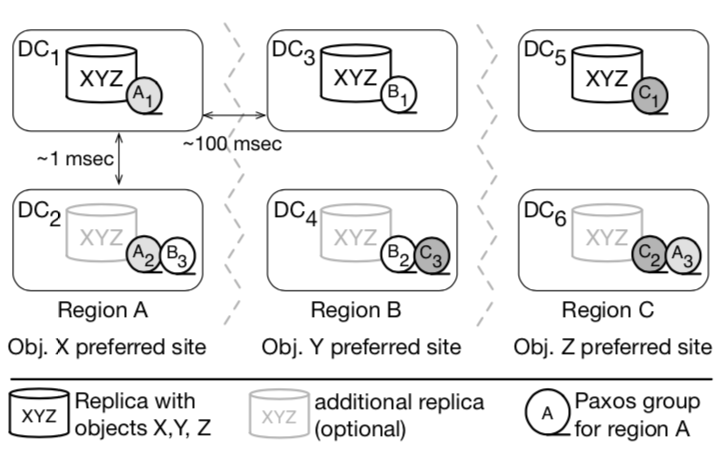
\includegraphics[width=\textwidth,height=\textheight,keepaspectratio]{img/datacenters.png}

  \caption{A possible deployment of GeoPaxos \citep{geopaxos}} 
  \label{fig:datacenters}
\end{figure}

Furthermore, GeoPaxos makes use of three important features that distinguish it from alternative solutions: these features are \emph{decoupling order from execution}, \emph{partial ordering of operations} and \emph{exploiting geographic locality}. 

% \clearpage
\subsection{Decoupling order from execution}
The Paxos protocol introduces a set of roles, namely acceptors, learners, proposers (and an eventual leader). When working with a distributed environment, deciding where to place each of these roles is important: in particular, placing acceptors and learners in the same replica, as it is often done, turns out not to be efficient. This is because we would want replicas to be close to the clients to decrease latency, but then the replicas would be far away from each other, increasing the latency required to perform the ordering of messages. Figure \ref{fig:decoupling_bad} shows such an example: the acceptors are forced to be far away to allow learners to be close to the clients, and putting the acceptors closer would cause the opposite problem.
\begin{figure}[htb]
  \centering
  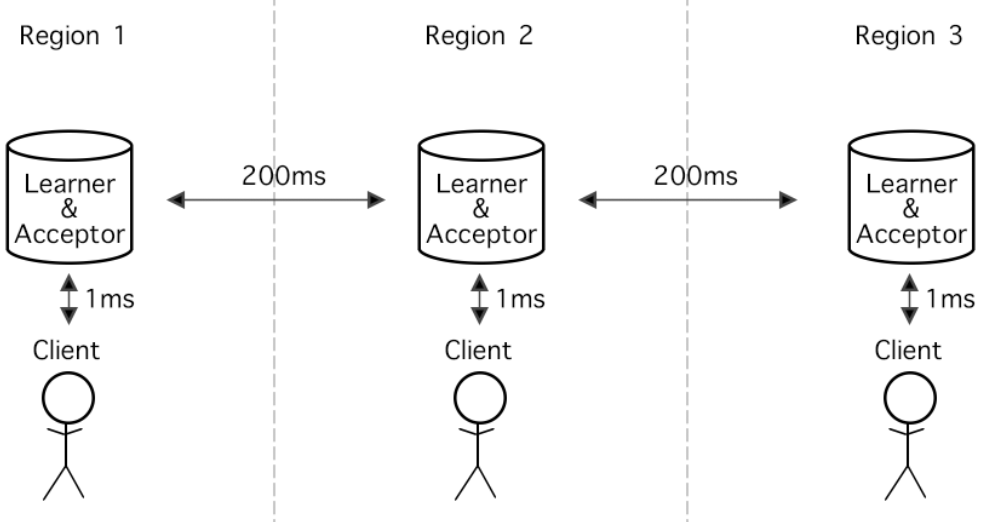
\includegraphics[width=\textwidth,height=\textheight,keepaspectratio]{img/decoupling_bad.png}
  \caption{A tyipical Paxos deployment which couples acceptors and learners}
  \label{fig:decoupling_bad}
\end{figure}

For this reason, GeoPaxos decouples the roles of acceptors and learners, which introduces a higher flexibility for the placement of the roles, allowing us to keep acceptor entities close to each other for the ordering communication and the learners close to the clients, so that their requests will be dispatched faster. Figure \ref{fig:decoupling_good} shows how this way we can deploy multiple acceptors in one region, which allows to avoid multi-region communications for single-group operations.

\begin{figure}[htb]
  \centering
  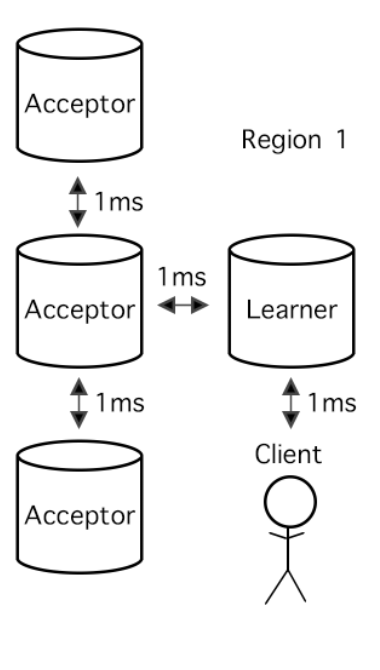
\includegraphics[width=0.32\textwidth,height=\textheight,keepaspectratio]{img/decoupling_good.png}
  \caption{A region with decoupled acceptor and learner entities}
  \label{fig:decoupling_good}
\end{figure}


% \begin{figure}
%   \centering
%   \begin{subfigure}[htb]
%     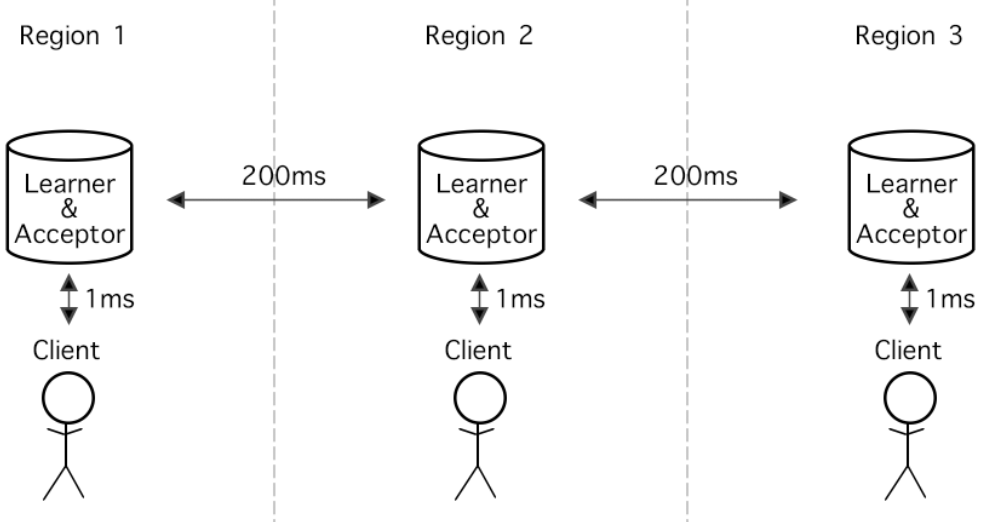
\includegraphics[width=\textwidth,height=\textheight,keepaspectratio]{img/decoupling_bad.png}
%   \end{subfigure}
  % \begin{subfigure}[htb]
  %   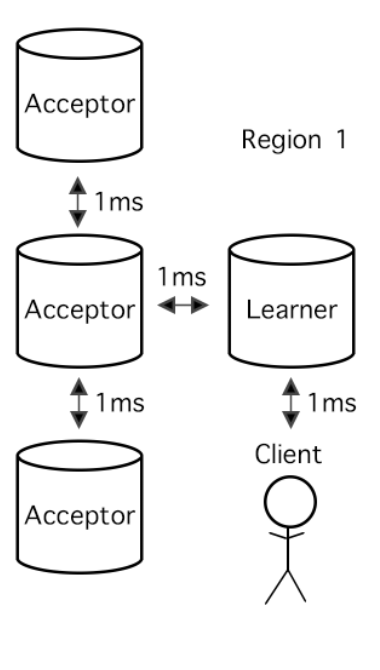
\includegraphics[width=\textwidth,height=\textheight,keepaspectratio]{img/decoupling_good.png}
  % \end{subfigure}
%   \caption{ A visualization of why coupling acceptors and learners is bad for performance. Placing the shared replica close to the clients forces the acceptors to be far apart, putting the acceptors close together makes the learners distant from the clients. Decoupling the two entities allows to have a learner and a quorum of acceptors in each region, allowing single-group operations to be performed efficiently. }
%   \label{fig:decoupling-bad}
% \end{figure}

% \begin{figure}[htb]
%   \centering
%   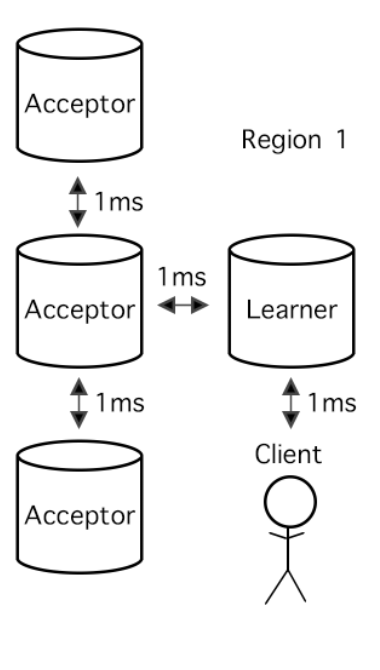
\includegraphics[width=\textwidth,height=\textheight,keepaspectratio]{img/decoupling_good.png}
%   \caption{ explanation }
%   \label{fig:decoupling-good}
% \end{figure}

\subsection{Partial ordering of operations}
The Paxos protocol allows us to impose a total order on all the messages ordered in the system. The issue is that this total ordering requires all the groups to communicate, slowing down the performance of the system. GeoPaxos handles this by only enforcing a partial order on messages.
A simple example of this can be seen where, for example, we have a sequence of various read operations on different objects. Since these operations do not alter the objects, we can perform them in different orders, as the state would remain consistent; but whenever we have a read and write on one object, these operations must be totally ordered.

Figure \ref{fig:partial-ordering} shows an example of commutative and non-commutative operations, respectively. In Figure (a) we have operations on two objects, $x$ and $y$, that do not conflict with each other, therefore the order of execution is not important. In Figure (b) instead we have conflicting operations that have to be ordered, which requires more communications to ensure the ordering.

\begin{figure}[htb]
  \centering
  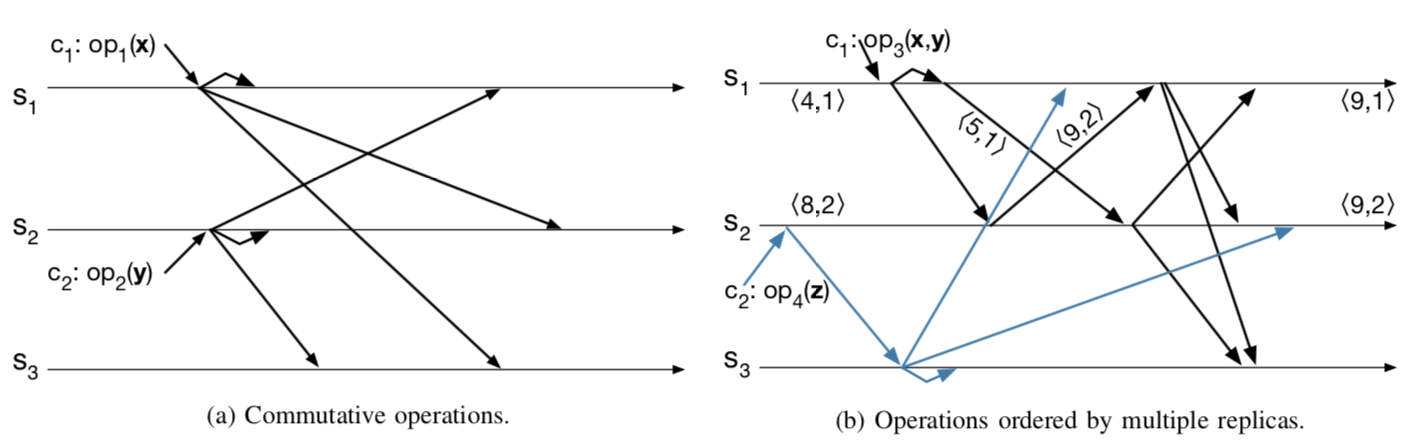
\includegraphics[width=\textwidth,height=\textheight,keepaspectratio]{img/partial-ordering.png}

  \caption{ Examples of commutative and non-commutative operations  \citep{geopaxos} }
  \label{fig:partial-ordering}
\end{figure}

\subsection{Exploiting geographic locality}
The third important feature of GeoPaxos is that it tries to exploit the geographic locality of the objects. Whenever clients perform operations on data objects of the system, we would often expect to see a certain degree of locality. In GeoPaxos the state and its objects are not sharded, but instead each object is handled by one or more groups, which means that operations must be ordered by said groups which can be placed in different geographic areas. This means that if we choose the groups that are closer to the region with the highest number of operations for each object, we will be able to reduce the latency for the majority of operations, improving the performance. Furthermore, if an object is handled by multiple groups but some operation does not conflict with other operations, then we will use the preferred partition, which is the closest group that has this object.